\documentclass[12pt,a4paper]{article}

\usepackage{style2017}
\newcounter{numexo}
\setcellgapes{1pt}
\renewcommand{\arraystretch}{1.2}
\setlength{\parskip}{0.25cm}

\begin{document}


\begin{NSI}
{Activité}{Feuille de style CSS}
\end{NSI}

%\section{Langage structuré}

\noindent L'image ci-dessous est notre premier document web écrit en langage html. Nous n'avons pas encore obtenu le résultat final attendu.

\begin{center}
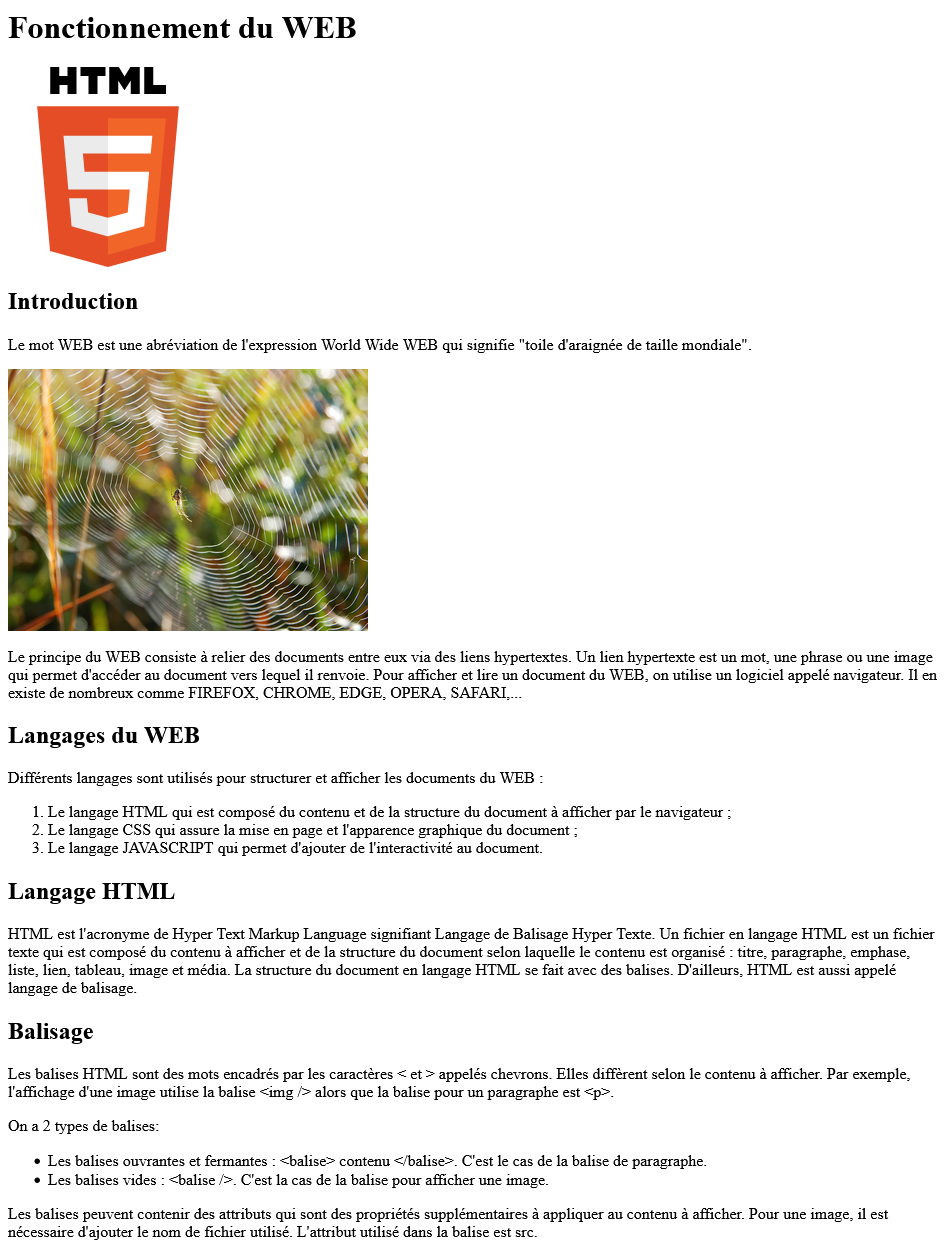
\includegraphics[scale=0.65]{img/style_css.png}
\end{center}

\newpage
Les améliorations à apporter ne relèvent pas du langage html mais des règles de style en CSS (Cascading Style Sheet) qui permet d'améliorer l'affichage graphique du document html.

Les règles de style CSS sont définies dans l'entête du document dans la balise \textsf{<head>}. Toutes les règles seront comprises entre les balises \textsf{<style>} et \textsf{</style>}. Cette balise doit contenir l'attribut \textsf{type} qui a pour valeur \textsf{"text/css"}.

Chaque règle peut être définie sur une balise html appelée alors \textbf{sélecteur}. Le sélecteur contient des propriétés auxquelles on associe des valeurs. Une règle CSS s'écrit toujours avec la même syntaxe : \begin{center}
\textsf{sélecteur\{propriété 1: valeur 1; propriété 2: valeur 2; \}}
\end{center}

Nous allons compléter notre document html pour appliquer les règles CSS qui vont nous permettre d'obtenir l'affichage souhaité.

\begin{enumerate}
\item Ajouter la balise de style dans votre document \textsf{html}.

\item Pour limiter la largeur de la page web et que celle-ci soit centrée, il faut ajouter les propriétés CSS suivantes sur le sélecteur \textsf{body}.

\begin{lstlisting}
	body{
		font-family: Verdana,sans-serif;
		font-size:1em;
		line-height:1.5em;
		width:1080px;
		margin:auto
	}
\end{lstlisting}

\item Le titre de la page \textsf{Fonctionnement du web} doit être centré et avoir une taille plus importante. 

Ajouter le sélecteur de titre, la propriété \textsf{text-align} qui a pour valeur \textsf{center} et la propriété \textsf{font-size} qui a pour valeur \textsf{3em}.

\item Les titres de niveau 2 ont une couleur bleue. La propriété CSS appropriée à la couleur est \textsf{color}. Les couleurs peuvent avoir plusieurs écritures.
\begin{itemize}[label=\textbullet]
\item le nom de la couleur en anglais,
\item le code couleur RGB en hexadécimal précédé du signe \#,
\item le code couleur RGB en décimal écrit entre parenthèses et précédé par \textsf{rgb}.
\end{itemize}
\begin{enumerate}
\item Quelles sont les trois écritures possibles pour la couleur bleu royal ?
\item Ajouter cette propriété CSS à votre document sous les trois dormes d'écritures.
\item Afficher les outils de développement du navigateur (F12) et inspecter l'un des titres de couleur bleue. Vérifier que la couleur ne change pas en activant ou désactivant les valeurs.
\end{enumerate}

\item Pour centrer une image sur une page, il faut appliquer les règles CSS sur le sélecteur \textsf{img} suivantes:
\begin{lstlisting}
	img{
		display:block;
		margin:16px auto;
	}
\end{lstlisting}
Ajouter cette règle pour centrer les images dans le document.


\newpage
\item La photo de toile d'araignée est encadrée avec un effet ombré. Pour obtenir cet effet, on applique les propriétés CSS suivantes:
\begin{lstlisting}
	border:solid 1px #eee;
	box-shadow:4px 4px #aaa;
	padding:8px;
\end{lstlisting}
\begin{enumerate}
\item Appliquer ces règles au sélecteur \textsf{img}. Que remarque-t-on ?
\item Pour éviter que des propriétés s'appliquent à tous les sélecteurs, on ajoute des \textsf{classes} aux sélecteurs. Il faut:
\begin{itemize}[label=\textbullet]
\item choisir un nom de classe qui regroupe les propriétés CSS,
\item ajouter au document html la classe dans le sélecteur où elle s'applique avec la syntaxe: \textsf{class="nom de la classe"} (pas de \textsf{'e'} à class),
\item ajouter dans la balise style la classe précédée d'un point avec toutes ces propriétés CSS.
\end{itemize}
Ajouter la classe \textsf{cadre} avec les propriétés CSS créant un cadre à la photo de toile d'araignée.
\end{enumerate}


\item Les styles CSS créés pour notre document ne sont applicables qu'à notre document. Si on souhaite appliquer les mêmes styles dans autre document html, il faudra ajouter ces styles.

C'est possible mais en cas de modification, il faudra modifier tous les documents html ce qui n'est pas optimal.

Pour éviter cela, on peut rassembler les propriétés CSS dans un fichier externe. Ce fichier est appelé feuille de style CSS et son extension est \textsf{css}.

\begin{enumerate}
\item Créer une feuille de style CSS qui comprend toutes les propriétés CSS de notre document et enregistrer cette feuille sous le nom \textsf{mon\_style.css}.
\item Remplacer dans votre document html, la balise \textsf{style} par la balise suivante:
\begin{center}
\textsf{<link type="text/css" href="mon\_style.css" rel="stylesheet" />}
\end{center}
\end{enumerate}

\item Ajouter un lien vers une feuille de style permet de créer des liens vers des feuilles de style se trouvant sur le web.

Un usage possible est l'application d'une police de style proposé par google. 
\begin{enumerate}
\item Rendez vous sur le site \url{https://fonts.google.com/},
\item Choisissez une police et copiez le lien de la feuille de style dans votre document.
\item Ajouter dans le sélecteur \textsf{body} la propriété CSS \textsf{font-family} associée.
\item Vérifiez que la police est bien appliquée à votre document html.
\end{enumerate}

\item Lorsque les propriétés CSS ont été appliquées, votre document doit ressembler à la capture suivante.
\end{enumerate}

\newpage
\begin{center}
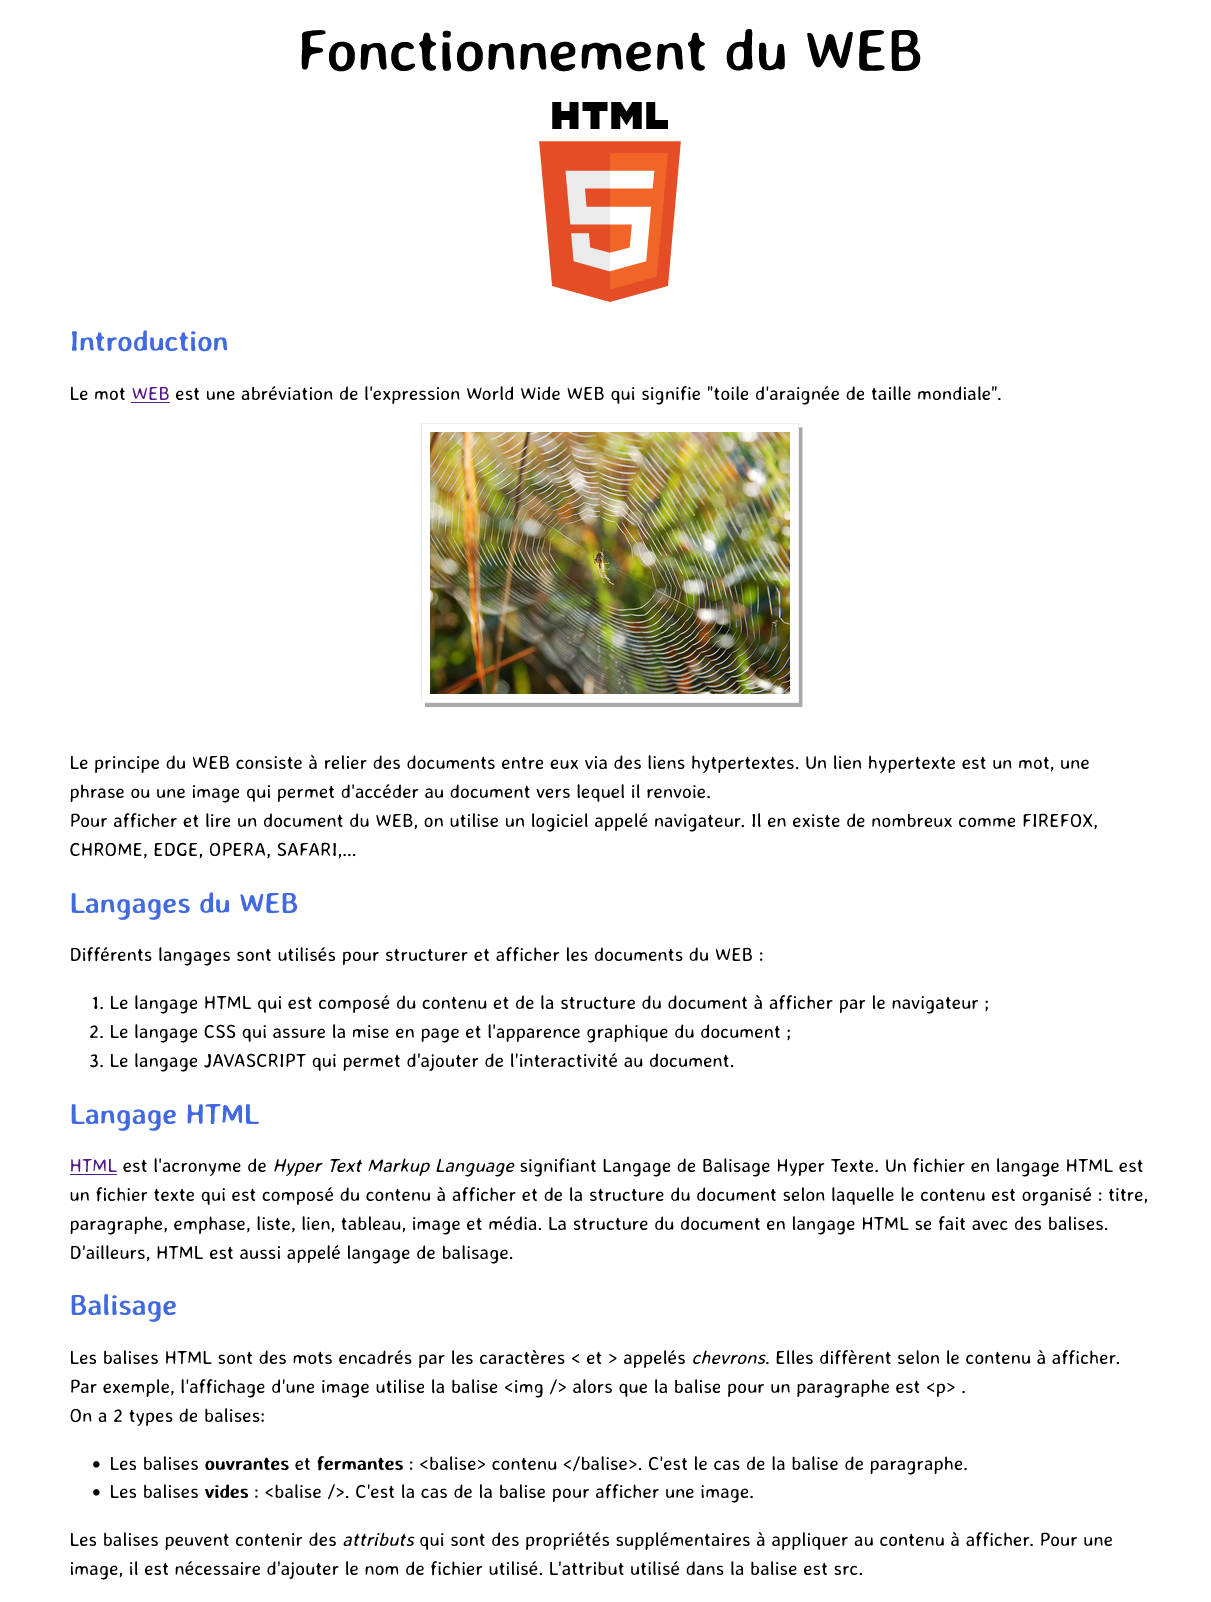
\includegraphics[scale=0.6]{img/activite_html.png}
\end{center}



\end{document}

